\chapter{Monitoring layer}\label{G:monitoringLayer}

As already discussed, in order to properly manage a cloud computing environment it is strongly required to use monitoring tools in order to gather information of interest by improving the environment itself or by finding out issues and solving them as fast as possible.

This chapter aims to showcase how the selected monitoring tools can fit in the architecture type that has been proposed and how they can be used. This means, preparing the environment to support Collectd (i.e.: monitoring and gathering) and Graphite (i.e.: storing and presenting) tools.

Moreover, to point out that such tools are helpful to demonstrate that LiveMediaStreamer framework could be deployed as the core of a real-time media production platform (see chapter \ref{H:platformDeploymentAndDemonstrations}).

So, to remark that the fact of creating small and reusable containers is the main goal of this chapter and, of course, the goal of this platform architecture to prototype. And, thanks to the selected monitoring tools, which are lightweight and ease configuration flexibility, this issue might be properly solved.

Then, a proposal of the monitoring architecture in a more detailed description (regarding figure \ref{F:MLAP}) is shown in figure \ref{F:maex}.

\begin{figure}[htb]
\begin{center}
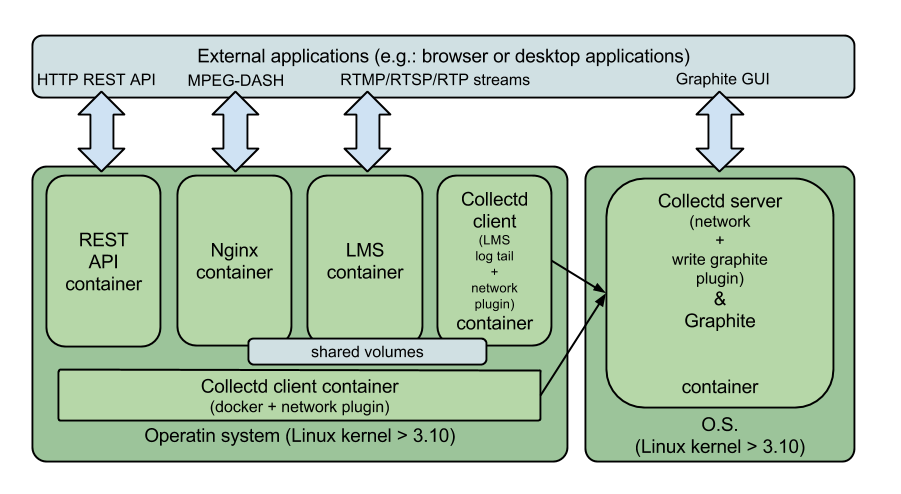
\includegraphics[width=0.9\textwidth]{./images/monitArchProp.png}
\caption{Detailed monitoring architecture}
\label{F:maex}
\end{center}
\end{figure}

Figure \ref{F:maex} showcases the relationship between different containers and the whole Collectd+Graphite deployment. Following sections are explaining it:

\section{Monitoring containers}

This section is based on how Collectd can be configured and deployed in order to monitor and properly gather metrics of interest.

\subsection{From container point of view}

From a container point of view and by following the premise to build containers as reusable as possible what is proposed to implement is a container that has the goal to gather the logged stats from an LMS container. This, as shown in figure \ref{F:maex}, implies sharing a Docker volume (as introduced in previous chapter \ref{D:virtualization}) from LMS container to the Collectd client which is using the tail plugin as an input. Moreover, in order to send specific logged metrics to the Collectd server container it is also using the network plugin as done in previous Collectd client configuration.

But, first of all, it is also required to be built in a container. This specific Docker file is shown in appendix \ref{ANX:dockerFiles} section \ref{ANX:dockerFiles5}.

Then, what is done in this case is to specify a bash script to run as CMD. This runs collectd but after envtpl python's package sets the environment parameters:
\begin{verbatim}
#!/bin/bash
envtpl /etc/collectd/collectd.conf.tpl
collectd -C /etc/collectd/collectd.conf -f
\end{verbatim}

Thanks to the envtpl package it is possible to run the container with specific environment variables in order to configure following parameters:

\begin{itemize}
\item LMS NAME \hfill

this will be used to identify the LMS instance in a container which Collectd is monitoring.
\item GRAPHITE HOST \hfill

this is to set the address of the remote/local container where the Collectd server is listening and pushing the metrics inside the Graphite's tools.
\item GRAPHITE PORT \hfill

this is the port where the Collect server and Graphite's tools container is listening to.
\end{itemize}

And these parameters are set in the Collectd configuration file as shown in appendix \ref{ANX:dockerFiles} section \ref{ANX:dockerFiles5} (among the specific plugins).

This Collectd configuration example file is loading specific system loggers plugins as inputs to be sent through the network plugin to the Collectd server.

But, in next chapter \ref{H:platformDeploymentAndDemonstrations} is shown an example of use of the Collectd tail plugin by using regular expressions. And this, as shown in figure \ref{F:maex}, this tail plugin is listening in an specific folder which is shared through the Docker's volume functionality with the LMS container, which logs its metrics in the same volume.

Finally, the Docker run command where the specific environment variables are set should be as shown next:
\begin{verbatim}
$ docker run -it -e "LMS_NAME=lms" \
	-e "GRAPHITE_HOST=<IP address>" -e "GRAPHITE_PORT=25826" \
	--rm --name cdc \
	-p 25826:25826/udp gerardcl/lms-collectd-client
\end{verbatim}

This will start immediately sending the defined container stats to the Graphite container specified by the environment parameters. Following section showcases the Graphite side to be deployed.

So, this example of deployed container for isolated Collectd clients is a key point in the general monitoring architecture due to the fact of being easyly configurable and reusable.

\subsection{From OS point of view}

The fact of using Collectd means a wide community behind, which probably have already developed required functionalities. And this is the case: in order to monitor each of the containers that a host OS might have it can be solved by configuring already existing plugins or similar tools for Collectd from Docker community. 

The selected tool is using the stats API introduced since Docker 1.5 version. And, the reported container's stats are:
 
\begin{itemize}
\item Network
\item Memory usage
\item CPU usage
\end{itemize}

The plugin is called "collectd-docker" and its documentation can be found in GitHub \cite{cdcontainer}. But, in order to follow the idea of clustering Collectd it has been modified in order to use the network plugin instead the write graphite plugin. So, the fact of being running on the same OS it requires changing the UDP ports through the metrics are sent by avoiding port binding issues. Moreover, previous Collectd client is also configured as a proxy server by re-configuring the network plugin as shown next: 

\begin{verbatim}
<Plugin network>
  Server "{{ GRAPHITE_HOST }}" "{{ GRAPHITE_PORT | default("25826") }}"
  Listen "*" "25827"
  Forward true
  ReportStats true
</Plugin>
\end{verbatim}

Therefore, it is not a plugin itself but a Docker container, which listens the docker daemon socket of the system (as proposed in figure \ref{F:maex}) and monitors each one of the containers running.

This container implements the same envtpl python package in order to define specific environment parameters such as the collectd server host and port (check its documentation for a detailed configuration explanation). So, in order to showcase how this and the previous Collect client are interconnected the following Docker run commands are shown:

\begin{itemize}
\item Collectd tail client (from the container point of view):
\begin{verbatim}
docker run -it --rm --name cc -v /home/gerardcl/logs/:/home/lms/logs \
-p 25826:25826/udp -e "LMS_NAME=lmsAVMixingStats" \
-e "GRAPHITE_HOST=192.168.1.140" \
gerardcl/lms-collectd-client
\end{verbatim}
\item Collectd docker socket API reader (from the OS point of view):
\begin{verbatim}
docker run -v /var/run/docker.sock:/var/run/docker.sock \
-e GRAPHITE_HOST=127.0.0.1 -e COLLECTD_HOST=lmsOS \
-e COLLECTD_DOCKER_APP=lmsAVMixStats -e GRAPHITE_PORT=25827 \
-it --rm --name collector --net="container:cc"  \
gerardcl/lms-collectd-collector
\end{verbatim}
\end{itemize}

So, here, what is done in order to avoid port binding issues is to setup the Docker collectd collector container to use the same network environment of the Collectd tail client.

\section{Showcasing monitoring}

This section is focused on the storage and presentation side of the metrics already logged and gathered.

So, as already introduced, this is proposed to be done within a container built with a Collectd server (network data inputs served to Graphite) and a Graphite system (storing and presenting stats).

As commonly said by the Collectd and Graphite community, installing and configuring Graphite isn't at all so easy than installing and configuring Collectd. This fact is shown in the Docker file of the \ref{ANX:dockerFiles} section \ref{ANX:dockerFiles6} in order to build such container, as shown in figure \ref{F:maex}.

In this case, specific "collectd" and "graphite" users are created (among other environment configurations as shown). Then, a bunch of different and specific configuration files for graphite are added (i.e.: ADD command) to their specific configuration folders. And, finally, specific command executions for database (i.e.: sqlite3 \cite{sqlite}, which is required for specific features for the Graphite web application) synchronization and other final configurations required for Graphite are also done. Regarding Collectd, it is installed in a similiar way as previously done but it is now configured as shown in \ref{ANX:dockerFiles} section \ref{ANX:collectdFiles2}.

So, here, Collectd is configured as a server by listening from anywhere at the default port for Collectd clustering. Moreover, the "write graphite" plugin is loaded in order to work as an output to the Graphite's Carbon tool, which receives the data to be stored in the Whisper RRD of the Graphite installation.

In this case, it is required to configure this container to be able to run multiple processes (i.e.: Graphite and Collectd). Therefore, by following previous section of how to run multiple processes inside a container in chapter \ref{D:virtualization}, the Supervisord system is used. This time it's configured by splitting the processes configurations into two parts, the Collectd and the Graphite. This last is configuring the Graphite web application and the Graphite's Carbon cache.

\begin{itemize}
\item Collectd: \hfill

\begin{verbatim}
[program:collectd]
user=collectd
directory=/
command=collectd -C /etc/collectd/collectd.conf -f
stdout_logfile=/var/log/supervisor/%(program_name)s.log
stderr_logfile=/var/log/supervisor/%(program_name)s_error.log
\end{verbatim}
\item Graphite web: \hfill

\begin{verbatim}
[program:graphite-web]
user=graphite
directory=/opt/graphite/webapp/
command=/opt/graphite/env/bin/gunicorn -w 1 -b 0.0.0.0:8080 \
	--pythonpath /opt/graphite/webapp/graphite graphite_wsgi
stdout_logfile=/var/log/supervisor/%(program_name)s.log
stderr_logfile=/var/log/supervisor/%(program_name)s_error.log
\end{verbatim}

\item Carbon cache: \hfill

\begin{verbatim}
[program:carbon-cache]
user=graphite
directory=/
env=PYTHONPATH=/opt/graphite/lib/
command=/opt/graphite/bin/carbon-cache.py --debug start
stdout_logfile=/var/log/supervisor/%(program_name)s.log
stderr_logfile=/var/log/supervisor/%(program_name)s_error.log
\end{verbatim}
\end{itemize}

An important configuration that must be decided and configured by knowing the requirements for why monitoring is required implies defining the storage schemas, which detail retention rates for storing metrics by following what was introduced in chapter \ref{B:problemStatementAndProposal}, the Round-Robin Database storage type. So, in order to work over a real-time media production platform it is important to achieve as much time accuracy as possible regarding the specific metrics of interest (e.g.: bandwidth usage, losses, pipeline delays, \ldots). There are more files regarding the Graphite's tools configuration too, but most of them are set to default values which are the recommended ones. 

Before going to present results and comment the outcomes (chapter \ref{H:platformDeploymentAndDemonstrations}), it is important to showcase example commands for both Collectd client and Collectd server + Graphite's containers:

\begin{verbatim}
$ docker run -it -e "LMS_NAME=lms" -e "GRAPHITE_HOST=<IP of >" \
--rm --name collectd -p 25826:25826/udp gerardcl/lms-collectd-client
\end{verbatim}

\begin{verbatim}
$ docker run -it --rm --name graphite -p 25826:25826/udp -p 8080:8080 \
gerardcl/lms-collectd-graphite
\end{verbatim}

As shown, the collectd (i.e.: Collectd client) container is sending to the default port (i.e.: UDP protocol) of the graphite host's (Collectd server and Graphite tools) container. Moreover, the graphite container opens HTTP port 8080 in order to enable browsers to get access to its web application anywhere. 
